\section[Venue applications]{Apply the Model: Two Outdoor Dining Venues}
\label{sec:applications}

\subsection{Different climates, the same service calculation}
We apply CP-SET to a dining sector of \textbf{Ullman Terrace at Desert Botanical Garden, Phoenix}, an outdoor event patio \cite{ullman}, and \textbf{Satay Street at Lau Pa Sat, Singapore}, an open-air dining street on Boon Tat Street \cite{satay-street}. Their dry-desert and humid-tropical climate contrast is represented by the warm-day scenarios in Table~\ref{tab:venue-inputs}.

Both spaces are open enough for a prescribed-background planning approximation. We retain the bus model's device outlets, enthalpy--moisture mixing, local-speed profiles and SET calculation, together with the station model's integer allocation and disjoint coverage. Three delivery strips within each device footprint represent attenuation from its near to far edge. Their equal-weight mean excess is $D_k=\frac13\sum_{j=1}^{3}D(\Theta_{kj})$. With the coverage fractions $c_{zk}$ from Eq.~\eqref{eq:coverage},
\begin{equation}
 \overline R_s=\frac{\sum_z n_z\left[(1-\sum_k c_{zk})D_0+
                  \sum_k c_{zk}D_k\right]}{\sum_z n_z},\qquad
 U_s=H\Big(\sum_z n_z\Big)(D_0-\overline R_s).
\label{eq:venue-service}
\end{equation}
Thus geometry controls who receives relief, while $E_s=H\sum_{z,k}x_{zk}p_k$ counts every device. The supply flow used for water demand belongs to each physical device, not separately to each delivery strip. Fixed background and $\chi=0$ retain the shelter approximation; crowd-driven accumulation or poorly flushed enclosures require the dynamic station equations instead.

\subsection{Climate changes the value of evaporation}
Task 3 ranks $\eta$ over every positive-energy layout satisfying nonoverlap: $12{,}166$ in Phoenix and $3{,}374$ in Singapore. \textbf{The maximum efficiencies are $81.10$ and $134.89$ person$\cdot{}^\circ$C$\cdot$h/kWh.} A single fan in the busiest zone attains each maximum, covering $10\%$ and $12.5\%$ of guest-time, respectively. Up to five such fans in Phoenix and four in Singapore tie while remaining inside that zone; no coverage, cost or residual threshold enters this efficiency ranking.

Table~\ref{tab:venue-results} separately compares pure types at the same coverage. Within each type, we choose the least-energy layout achieving that coverage. The wet-bulb temperatures are $20.90^\circ$C in Phoenix and $28.16^\circ$C in Singapore. Consequently, C achieves its $8^\circ$C outlet-drop cap in the dry scenario, but only $2.68^\circ$C in the humid scenario. Dilution and the SET response translate this outlet change into useful service.

\begin{table}[!ht]
\centering\small
\caption{Equal-coverage efficiency comparison: every plan serves $60\%$ of guest-time. $U$ is person$\cdot{}^\circ$C$\cdot$h and $\eta=U/E$.}
\label{tab:venue-results}
\begin{tabular}{@{}llrrr@{}}
\toprule
Venue & Plan & $U$ & $E$ (kWh) & $\eta$\\
\midrule
Phoenix & A7 & 486.58 & 7.0 & 69.51\\
 & B5 & 666.41 & 24.0 & 27.77\\
 & C4 & 1183.98 & 40.0 & 29.60\\
Singapore & A6 & 647.48 & 6.0 & 107.91\\
 & B4 & 728.44 & 19.2 & 37.94\\
 & C3 & 1069.98 & 30.0 & 35.67\\
\bottomrule
\end{tabular}
\end{table}

Fans give the greatest service per kWh in both comparisons. The B--C efficiency order reverses: C exceeds B in Phoenix, whereas B exceeds C in Singapore. Humidity removes C's larger outlet-temperature-drop advantage, leaving delivery reach and unit power to determine its efficiency. Singapore's larger fan efficiency also reflects its denser dining sector and stronger modeled SET response to air movement. Occupancy, delivery and climate therefore belong in the same calculation.

\begin{figure}[!ht]
\centering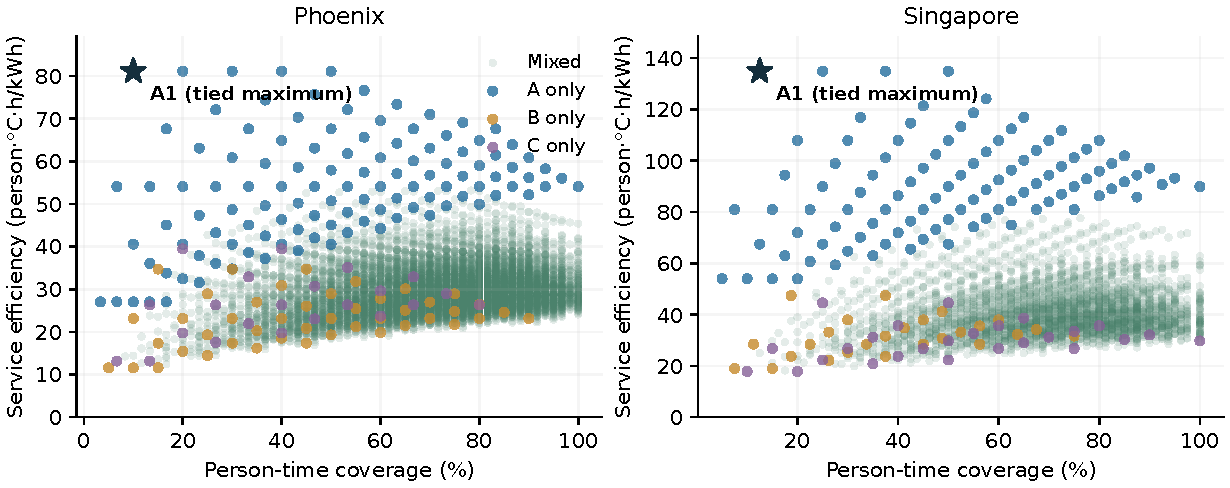
\includegraphics[width=\linewidth]{figures/27_venue_comparison.pdf}
\caption{Efficiency over all positive-energy integer layouts, with no coverage threshold. Coincident points are merged for display. Stars identify the smallest installations attaining the tied maximum; broader service changes the relevant occupied locations.}
\label{fig:venue-comparison}
\end{figure}

\subsection{What scales, and what does not}
Efficient cooling depends chiefly on delivering air to occupied locations, preserving useful speed, limiting dilution, and exploiting a sufficient dry-bulb--wet-bulb difference. Increasing area changes the equipment count and occupied-location weights; it does not multiply $\eta$ directly.

A scale check makes this distinction concrete. Doubling Singapore's area and guests at the same density, while retaining the reference fan layout $(4,4,2)$, leaves $U/E=97.12$ unchanged but halves coverage from $90\%$ to $45\%$. Doubling the devices as well restores coverage, doubles electricity from $10$ to $20$ kWh, and again preserves $U/E$. Efficiency is therefore an intensity measure; service adequacy enters the next task. The code verifies these scaling identities, $U+R=R_0$, saturation bounds and the shared heat/moisture conservation checks.

